%%%%%%%%%%%%%%%%%%%%%%%%%%%%%%%%%%%%%%%%%%%%%%%%%%%%%%%%%%%%%%%%%%%%%%%%%%%%%%%
\chapter{Lei de Hooke}
\label{Chap:ExpLeiDeHooke}
%%%%%%%%%%%%%%%%%%%%%%%%%%%%%%%%%%%%%%%%%%%%%%%%%%%%%%%%%%%%%%%%%%%%%%%%%%%%%%%

\begin{fullwidth}\it
	Realizaremos um experimento em que submeteremos uma mola a forças com intensidades diferentes, observando as distensões correspondentes. Procuramos assim observar experimentalmente a Lei de Hooke --- que afirma que as distensões são diretamente proporcionais à intensidade da força aplicada ---. Utilizaremos os seguintes conceitos: medidas, algarismos significativos, gráficos, e regressão linear.
\end{fullwidth}

%%%%%%%%%%%%%%%%%%%%%%%%%%%%%%%%%%%%%%%%%%%%%%%%
\section[Linhas de tendência e regressão linear]{Linhas de tendência e regressão linear\footnote{Esta seção é um resumo do Capítulo~\ref{Chap:RegressoLinear}.}}
%%%%%%%%%%%%%%%%%%%%%%%%%%%%%%%%%%%%%%%%%%%%%%%%

Quando realizamos um experimento, procuramos relacionar uma variável dependente a uma variável independente. Para visualizarmos a relação entre as duas, é interessante fazer uma representação gráfica da variável dependente em função dos valores da variável independente. Podemos assim verificar uma tendência geral dos pontos, que pode seguir padrões retilíneos, parabólicos, etc. Muitas vezes tal padrão é muito claro, pois os pontos tem uma \emph{dispersão} baixa. Outras vezes a dispersão é razoavelmente alta e fica difícil verificar o padrão seguido pelos pontos.

Mesmo em casos em que podemos verificar um padrão aparente ao fazer um gráfico, determinar a forma mais adequada para a \emph{linha de tendência} que melhor descreve os pontos experimentais ---~ou mesmo afirmar que tais pontos seguem este padrão~--- pode ser complicado. Se, por exemplo, fizermos uma série de medidas que seguem um padrão parabólico, mas com medidas que se restringem a um intervalo pequeno da variável independente, o gráfico terá a aparência de uma reta.

Determinar o padrão seguido pelos pontos, é, portanto, uma tarefa que não pode ser feita a partir de um gráfico: o mais adequado é termos uma \emph{teoria acerca do fenômeno físico} que descreva qual é o padrão que os pontos devem seguir, e usar um gráfico para determinar se tal descrição é coerente. Verificaremos posteriormente como determinar se uma teoria é plausível ou não, por hora vamos nos preocupar em determinar a \emph{melhor reta} que ajusta um conjunto de dados.

Sempre que tivermos um conjunto de dados, podemos calcular a melhor reta que o representa através de um processo de \emph{regressão linear}. Este processo consiste em aplicar um método matemático que tome os dados experimentais e calcule os coeficientes linear $A$ e angular $B$ para a equação da reta:
\begin{equation}
	y = A + Bx.
\end{equation}

%%%%%%%%%%%%%%%%%%%%%%%%%%%%%
\paragraph{Mínimos quadrados}
%%%%%%%%%%%%%%%%%%%%%%%%%%%%%

O método utilizado para obter tais coeficientes é o de \emph{mínimos quadrados}. Nele, são encontrados os coeficientes de forma a minimizar o quadrado da distância entre os pontos experimentais e a ``melhor reta''. É possível mostrar\cite{Taylor}, utilizando técnicas de cálculo, que para minimizarmos a soma do quadrado das distâncias entre os pontos e a melhor reta, os coeficientes linear e angular são dados por
\begin{align}
	A &= \frac{\sum x_i^2 \sum y_i - \sum x_i \sum x_iy_i}{N \sum x_i^2 - (\sum x_i)^2} \\
	B &= \frac{N\sum x_iy_i - \sum x_i \sum y_i}{N \sum x_i^2 - (\sum x_i)^2}.
\end{align}
%
onde as somas se dão sobre todas mas medidas $x_i$ e $y_i$, $N$ representa o número de medidas, e as médias das medidas para as variáveis $x$ e $y$ são representadas por $\mean{x}$ e $\mean{y}$, respectivamente. Após fazer a regressão, podemos utilizar os coeficientes para traçar as \emph{retas de tendência} nos gráficos\footnote{Quando tais retas forem calculadas, adicione as equações resultantes aos gráficos.}.

Ao fazermos o processo de regressão linear, a calculadora também calculará o \emph{coeficiente de correlação linear} $r$, dado por
\begin{equation}
	r = \frac{\sum (x_i - \mean{x})(y_i-\mean{y})}{\sqrt{\sum(x_i - \mean{x})^2\sum (y_i - \mean{y})^2}}.
\end{equation}
%
Tal coeficiente pode ser interpretado como um ``índice de confiança'' e geralmente é calculado ao quadrado, pois seus valores podem variar entre $-1$ e $1$. Quanto mais próximo $r$ for de $\pm 1$, menor é a dispersão dos pontos em relação ao comportamento retilíneo, ou seja, maiores são as chances de que o fenômeno estudado e que deu origem aos dados siga uma relação linear. Este número geralmente se parece com algo como $r^2=\np{0,99998}$, $r^2=\np{0,997}$, $r^2= \np{0,990}$, etc., quando os dados são altamente lineares e relativamente abundantes. Se a dispersão em relação ao comportamento linear for grande e forem poucos os pontos, $r^2$ pode cair para \np{0,7}, ou valores menores.

\begin{figure}[!h]
\centering
\begin{tikzpicture}[gnuplot]
%% generated with GNUPLOT 5.0p0 (Lua 5.3; terminal rev. 99, script rev. 100)
%% 2015-05-18T22:58:50 BRT
\path (0.000,0.000) rectangle (14.000,9.000);
\gpcolor{color=gp lt color border}
\gpsetlinetype{gp lt border}
\gpsetdashtype{gp dt solid}
\gpsetlinewidth{1.00}
\draw[gp path] (1.320,2.077)--(1.500,2.077);
\draw[gp path] (13.447,2.077)--(13.267,2.077);
\node[gp node right] at (1.136,2.077) {$20$};
\draw[gp path] (1.320,3.534)--(1.500,3.534);
\draw[gp path] (13.447,3.534)--(13.267,3.534);
\node[gp node right] at (1.136,3.534) {$40$};
\draw[gp path] (1.320,4.990)--(1.500,4.990);
\draw[gp path] (13.447,4.990)--(13.267,4.990);
\node[gp node right] at (1.136,4.990) {$60$};
\draw[gp path] (1.320,6.446)--(1.500,6.446);
\draw[gp path] (13.447,6.446)--(13.267,6.446);
\node[gp node right] at (1.136,6.446) {$80$};
\draw[gp path] (1.320,7.903)--(1.500,7.903);
\draw[gp path] (13.447,7.903)--(13.267,7.903);
\node[gp node right] at (1.136,7.903) {$100$};
\draw[gp path] (1.711,0.985)--(1.711,1.165);
\draw[gp path] (1.711,8.631)--(1.711,8.451);
\node[gp node center] at (1.711,0.677) {$0$};
\draw[gp path] (3.667,0.985)--(3.667,1.165);
\draw[gp path] (3.667,8.631)--(3.667,8.451);
\node[gp node center] at (3.667,0.677) {$5$};
\draw[gp path] (5.623,0.985)--(5.623,1.165);
\draw[gp path] (5.623,8.631)--(5.623,8.451);
\node[gp node center] at (5.623,0.677) {$10$};
\draw[gp path] (7.579,0.985)--(7.579,1.165);
\draw[gp path] (7.579,8.631)--(7.579,8.451);
\node[gp node center] at (7.579,0.677) {$15$};
\draw[gp path] (9.535,0.985)--(9.535,1.165);
\draw[gp path] (9.535,8.631)--(9.535,8.451);
\node[gp node center] at (9.535,0.677) {$20$};
\draw[gp path] (11.491,0.985)--(11.491,1.165);
\draw[gp path] (11.491,8.631)--(11.491,8.451);
\node[gp node center] at (11.491,0.677) {$25$};
\draw[gp path] (13.447,0.985)--(13.447,1.165);
\draw[gp path] (13.447,8.631)--(13.447,8.451);
\node[gp node center] at (13.447,0.677) {$30$};
\draw[gp path] (1.320,8.631)--(1.320,0.985)--(13.447,0.985)--(13.447,8.631)--cycle;
\node[gp node center,rotate=-270] at (0.246,4.808) {$y_1$};
\node[gp node center] at (7.383,0.215) {$x$};
\node[gp node left] at (2.788,8.297) {Dados experimentais};
\gpcolor{rgb color={0.000,0.000,0.000}}
\gpsetlinewidth{2.00}
\gpsetpointsize{4.00}
\gppoint{gp mark 7}{(1.990,1.682)}
\gppoint{gp mark 7}{(2.765,2.128)}
\gppoint{gp mark 7}{(3.428,2.458)}
\gppoint{gp mark 7}{(3.652,2.620)}
\gppoint{gp mark 7}{(4.154,2.823)}
\gppoint{gp mark 7}{(4.558,3.051)}
\gppoint{gp mark 7}{(4.676,3.111)}
\gppoint{gp mark 7}{(4.731,3.222)}
\gppoint{gp mark 7}{(4.806,3.170)}
\gppoint{gp mark 7}{(4.950,3.354)}
\gppoint{gp mark 7}{(5.245,3.577)}
\gppoint{gp mark 7}{(5.405,3.472)}
\gppoint{gp mark 7}{(5.743,3.769)}
\gppoint{gp mark 7}{(5.847,3.709)}
\gppoint{gp mark 7}{(6.084,3.883)}
\gppoint{gp mark 7}{(7.710,4.816)}
\gppoint{gp mark 7}{(8.370,5.269)}
\gppoint{gp mark 7}{(9.115,5.577)}
\gppoint{gp mark 7}{(9.773,6.039)}
\gppoint{gp mark 7}{(9.878,6.088)}
\gppoint{gp mark 7}{(9.963,6.100)}
\gppoint{gp mark 7}{(10.406,6.246)}
\gppoint{gp mark 7}{(10.477,6.523)}
\gppoint{gp mark 7}{(10.501,6.361)}
\gppoint{gp mark 7}{(10.739,6.498)}
\gppoint{gp mark 7}{(12.047,7.279)}
\gppoint{gp mark 7}{(12.220,7.304)}
\gppoint{gp mark 7}{(12.414,7.414)}
\gppoint{gp mark 7}{(2.146,8.297)}
\gpcolor{color=gp lt color border}
\node[gp node left] at (2.788,7.989) {$y(x)=\np{2.9844463644}x + \np{12.141173236}$, $r^2 = \np{0.9989011203}$};
\gpcolor{rgb color={0.000,0.000,0.000}}
\draw[gp path] (1.688,7.989)--(2.604,7.989);
\draw[gp path] (1.908,1.614)--(1.914,1.618)--(1.920,1.621)--(1.926,1.625)--(1.932,1.628)%
  --(1.938,1.631)--(1.945,1.635)--(1.951,1.638)--(1.957,1.641)--(1.963,1.645)--(1.969,1.648)%
  --(1.975,1.651)--(1.981,1.655)--(1.987,1.658)--(1.993,1.662)--(1.999,1.665)--(2.005,1.668)%
  --(2.011,1.672)--(2.017,1.675)--(2.023,1.678)--(2.029,1.682)--(2.035,1.685)--(2.042,1.689)%
  --(2.048,1.692)--(2.054,1.695)--(2.060,1.699)--(2.066,1.702)--(2.072,1.705)--(2.078,1.709)%
  --(2.084,1.712)--(2.090,1.715)--(2.096,1.719)--(2.102,1.722)--(2.108,1.726)--(2.114,1.729)%
  --(2.120,1.732)--(2.126,1.736)--(2.133,1.739)--(2.139,1.742)--(2.145,1.746)--(2.151,1.749)%
  --(2.157,1.753)--(2.163,1.756)--(2.169,1.759)--(2.175,1.763)--(2.181,1.766)--(2.187,1.769)%
  --(2.193,1.773)--(2.199,1.776)--(2.205,1.779)--(2.211,1.783)--(2.217,1.786)--(2.223,1.790)%
  --(2.230,1.793)--(2.236,1.796)--(2.242,1.800)--(2.248,1.803)--(2.254,1.806)--(2.260,1.810)%
  --(2.266,1.813)--(2.272,1.817)--(2.278,1.820)--(2.284,1.823)--(2.290,1.827)--(2.296,1.830)%
  --(2.302,1.833)--(2.308,1.837)--(2.314,1.840)--(2.320,1.843)--(2.327,1.847)--(2.333,1.850)%
  --(2.339,1.854)--(2.345,1.857)--(2.351,1.860)--(2.357,1.864)--(2.363,1.867)--(2.369,1.870)%
  --(2.375,1.874)--(2.381,1.877)--(2.387,1.881)--(2.393,1.884)--(2.399,1.887)--(2.405,1.891)%
  --(2.411,1.894)--(2.417,1.897)--(2.424,1.901)--(2.430,1.904)--(2.436,1.907)--(2.442,1.911)%
  --(2.448,1.914)--(2.454,1.918)--(2.460,1.921)--(2.466,1.924)--(2.472,1.928)--(2.478,1.931)%
  --(2.484,1.934)--(2.490,1.938)--(2.496,1.941)--(2.502,1.945)--(2.508,1.948)--(2.515,1.951)%
  --(2.521,1.955)--(2.527,1.958)--(2.533,1.961)--(2.539,1.965)--(2.545,1.968)--(2.551,1.972)%
  --(2.557,1.975)--(2.563,1.978)--(2.569,1.982)--(2.575,1.985)--(2.581,1.988)--(2.587,1.992)%
  --(2.593,1.995)--(2.599,1.998)--(2.605,2.002)--(2.612,2.005)--(2.618,2.009)--(2.624,2.012)%
  --(2.630,2.015)--(2.636,2.019)--(2.642,2.022)--(2.648,2.025)--(2.654,2.029)--(2.660,2.032)%
  --(2.666,2.036)--(2.672,2.039)--(2.678,2.042)--(2.684,2.046)--(2.690,2.049)--(2.696,2.052)%
  --(2.702,2.056)--(2.709,2.059)--(2.715,2.062)--(2.721,2.066)--(2.727,2.069)--(2.733,2.073)%
  --(2.739,2.076)--(2.745,2.079)--(2.751,2.083)--(2.757,2.086)--(2.763,2.089)--(2.769,2.093)%
  --(2.775,2.096)--(2.781,2.100)--(2.787,2.103)--(2.793,2.106)--(2.799,2.110)--(2.806,2.113)%
  --(2.812,2.116)--(2.818,2.120)--(2.824,2.123)--(2.830,2.126)--(2.836,2.130)--(2.842,2.133)%
  --(2.848,2.137)--(2.854,2.140)--(2.860,2.143)--(2.866,2.147)--(2.872,2.150)--(2.878,2.153)%
  --(2.884,2.157)--(2.890,2.160)--(2.897,2.164)--(2.903,2.167)--(2.909,2.170)--(2.915,2.174)%
  --(2.921,2.177)--(2.927,2.180)--(2.933,2.184)--(2.939,2.187)--(2.945,2.190)--(2.951,2.194)%
  --(2.957,2.197)--(2.963,2.201)--(2.969,2.204)--(2.975,2.207)--(2.981,2.211)--(2.987,2.214)%
  --(2.994,2.217)--(3.000,2.221)--(3.006,2.224)--(3.012,2.228)--(3.018,2.231)--(3.024,2.234)%
  --(3.030,2.238)--(3.036,2.241)--(3.042,2.244)--(3.048,2.248)--(3.054,2.251)--(3.060,2.254)%
  --(3.066,2.258)--(3.072,2.261)--(3.078,2.265)--(3.084,2.268)--(3.091,2.271)--(3.097,2.275)%
  --(3.103,2.278)--(3.109,2.281)--(3.115,2.285)--(3.121,2.288)--(3.127,2.292)--(3.133,2.295)%
  --(3.139,2.298)--(3.145,2.302)--(3.151,2.305)--(3.157,2.308)--(3.163,2.312)--(3.169,2.315)%
  --(3.175,2.318)--(3.181,2.322)--(3.188,2.325)--(3.194,2.329)--(3.200,2.332)--(3.206,2.335)%
  --(3.212,2.339)--(3.218,2.342)--(3.224,2.345)--(3.230,2.349)--(3.236,2.352)--(3.242,2.356)%
  --(3.248,2.359)--(3.254,2.362)--(3.260,2.366)--(3.266,2.369)--(3.272,2.372)--(3.279,2.376)%
  --(3.285,2.379)--(3.291,2.382)--(3.297,2.386)--(3.303,2.389)--(3.309,2.393)--(3.315,2.396)%
  --(3.321,2.399)--(3.327,2.403)--(3.333,2.406)--(3.339,2.409)--(3.345,2.413)--(3.351,2.416)%
  --(3.357,2.420)--(3.363,2.423)--(3.369,2.426)--(3.376,2.430)--(3.382,2.433)--(3.388,2.436)%
  --(3.394,2.440)--(3.400,2.443)--(3.406,2.446)--(3.412,2.450)--(3.418,2.453)--(3.424,2.457)%
  --(3.430,2.460)--(3.436,2.463)--(3.442,2.467)--(3.448,2.470)--(3.454,2.473)--(3.460,2.477)%
  --(3.466,2.480)--(3.473,2.484)--(3.479,2.487)--(3.485,2.490)--(3.491,2.494)--(3.497,2.497)%
  --(3.503,2.500)--(3.509,2.504)--(3.515,2.507)--(3.521,2.510)--(3.527,2.514)--(3.533,2.517)%
  --(3.539,2.521)--(3.545,2.524)--(3.551,2.527)--(3.557,2.531)--(3.563,2.534)--(3.570,2.537)%
  --(3.576,2.541)--(3.582,2.544)--(3.588,2.548)--(3.594,2.551)--(3.600,2.554)--(3.606,2.558)%
  --(3.612,2.561)--(3.618,2.564)--(3.624,2.568)--(3.630,2.571)--(3.636,2.574)--(3.642,2.578)%
  --(3.648,2.581)--(3.654,2.585)--(3.661,2.588)--(3.667,2.591)--(3.673,2.595)--(3.679,2.598)%
  --(3.685,2.601)--(3.691,2.605)--(3.697,2.608)--(3.703,2.612)--(3.709,2.615)--(3.715,2.618)%
  --(3.721,2.622)--(3.727,2.625)--(3.733,2.628)--(3.739,2.632)--(3.745,2.635)--(3.751,2.638)%
  --(3.758,2.642)--(3.764,2.645)--(3.770,2.649)--(3.776,2.652)--(3.782,2.655)--(3.788,2.659)%
  --(3.794,2.662)--(3.800,2.665)--(3.806,2.669)--(3.812,2.672)--(3.818,2.676)--(3.824,2.679)%
  --(3.830,2.682)--(3.836,2.686)--(3.842,2.689)--(3.848,2.692)--(3.855,2.696)--(3.861,2.699)%
  --(3.867,2.702)--(3.873,2.706)--(3.879,2.709)--(3.885,2.713)--(3.891,2.716)--(3.897,2.719)%
  --(3.903,2.723)--(3.909,2.726)--(3.915,2.729)--(3.921,2.733)--(3.927,2.736)--(3.933,2.740)%
  --(3.939,2.743)--(3.945,2.746)--(3.952,2.750)--(3.958,2.753)--(3.964,2.756)--(3.970,2.760)%
  --(3.976,2.763)--(3.982,2.766)--(3.988,2.770)--(3.994,2.773)--(4.000,2.777)--(4.006,2.780)%
  --(4.012,2.783)--(4.018,2.787)--(4.024,2.790)--(4.030,2.793)--(4.036,2.797)--(4.043,2.800)%
  --(4.049,2.804)--(4.055,2.807)--(4.061,2.810)--(4.067,2.814)--(4.073,2.817)--(4.079,2.820)%
  --(4.085,2.824)--(4.091,2.827)--(4.097,2.830)--(4.103,2.834)--(4.109,2.837)--(4.115,2.841)%
  --(4.121,2.844)--(4.127,2.847)--(4.133,2.851)--(4.140,2.854)--(4.146,2.857)--(4.152,2.861)%
  --(4.158,2.864)--(4.164,2.868)--(4.170,2.871)--(4.176,2.874)--(4.182,2.878)--(4.188,2.881)%
  --(4.194,2.884)--(4.200,2.888)--(4.206,2.891)--(4.212,2.894)--(4.218,2.898)--(4.224,2.901)%
  --(4.230,2.905)--(4.237,2.908)--(4.243,2.911)--(4.249,2.915)--(4.255,2.918)--(4.261,2.921)%
  --(4.267,2.925)--(4.273,2.928)--(4.279,2.932)--(4.285,2.935)--(4.291,2.938)--(4.297,2.942)%
  --(4.303,2.945)--(4.309,2.948)--(4.315,2.952)--(4.321,2.955)--(4.327,2.958)--(4.334,2.962)%
  --(4.340,2.965)--(4.346,2.969)--(4.352,2.972)--(4.358,2.975)--(4.364,2.979)--(4.370,2.982)%
  --(4.376,2.985)--(4.382,2.989)--(4.388,2.992)--(4.394,2.996)--(4.400,2.999)--(4.406,3.002)%
  --(4.412,3.006)--(4.418,3.009)--(4.425,3.012)--(4.431,3.016)--(4.437,3.019)--(4.443,3.022)%
  --(4.449,3.026)--(4.455,3.029)--(4.461,3.033)--(4.467,3.036)--(4.473,3.039)--(4.479,3.043)%
  --(4.485,3.046)--(4.491,3.049)--(4.497,3.053)--(4.503,3.056)--(4.509,3.060)--(4.515,3.063)%
  --(4.522,3.066)--(4.528,3.070)--(4.534,3.073)--(4.540,3.076)--(4.546,3.080)--(4.552,3.083)%
  --(4.558,3.086)--(4.564,3.090)--(4.570,3.093)--(4.576,3.097)--(4.582,3.100)--(4.588,3.103)%
  --(4.594,3.107)--(4.600,3.110)--(4.606,3.113)--(4.612,3.117)--(4.619,3.120)--(4.625,3.124)%
  --(4.631,3.127)--(4.637,3.130)--(4.643,3.134)--(4.649,3.137)--(4.655,3.140)--(4.661,3.144)%
  --(4.667,3.147)--(4.673,3.150)--(4.679,3.154)--(4.685,3.157)--(4.691,3.161)--(4.697,3.164)%
  --(4.703,3.167)--(4.709,3.171)--(4.716,3.174)--(4.722,3.177)--(4.728,3.181)--(4.734,3.184)%
  --(4.740,3.188)--(4.746,3.191)--(4.752,3.194)--(4.758,3.198)--(4.764,3.201)--(4.770,3.204)%
  --(4.776,3.208)--(4.782,3.211)--(4.788,3.214)--(4.794,3.218)--(4.800,3.221)--(4.807,3.225)%
  --(4.813,3.228)--(4.819,3.231)--(4.825,3.235)--(4.831,3.238)--(4.837,3.241)--(4.843,3.245)%
  --(4.849,3.248)--(4.855,3.252)--(4.861,3.255)--(4.867,3.258)--(4.873,3.262)--(4.879,3.265)%
  --(4.885,3.268)--(4.891,3.272)--(4.897,3.275)--(4.904,3.278)--(4.910,3.282)--(4.916,3.285)%
  --(4.922,3.289)--(4.928,3.292)--(4.934,3.295)--(4.940,3.299)--(4.946,3.302)--(4.952,3.305)%
  --(4.958,3.309)--(4.964,3.312)--(4.970,3.316)--(4.976,3.319)--(4.982,3.322)--(4.988,3.326)%
  --(4.994,3.329)--(5.001,3.332)--(5.007,3.336)--(5.013,3.339)--(5.019,3.342)--(5.025,3.346)%
  --(5.031,3.349)--(5.037,3.353)--(5.043,3.356)--(5.049,3.359)--(5.055,3.363)--(5.061,3.366)%
  --(5.067,3.369)--(5.073,3.373)--(5.079,3.376)--(5.085,3.380)--(5.091,3.383)--(5.098,3.386)%
  --(5.104,3.390)--(5.110,3.393)--(5.116,3.396)--(5.122,3.400)--(5.128,3.403)--(5.134,3.406)%
  --(5.140,3.410)--(5.146,3.413)--(5.152,3.417)--(5.158,3.420)--(5.164,3.423)--(5.170,3.427)%
  --(5.176,3.430)--(5.182,3.433)--(5.189,3.437)--(5.195,3.440)--(5.201,3.444)--(5.207,3.447)%
  --(5.213,3.450)--(5.219,3.454)--(5.225,3.457)--(5.231,3.460)--(5.237,3.464)--(5.243,3.467)%
  --(5.249,3.470)--(5.255,3.474)--(5.261,3.477)--(5.267,3.481)--(5.273,3.484)--(5.279,3.487)%
  --(5.286,3.491)--(5.292,3.494)--(5.298,3.497)--(5.304,3.501)--(5.310,3.504)--(5.316,3.508)%
  --(5.322,3.511)--(5.328,3.514)--(5.334,3.518)--(5.340,3.521)--(5.346,3.524)--(5.352,3.528)%
  --(5.358,3.531)--(5.364,3.534)--(5.370,3.538)--(5.376,3.541)--(5.383,3.545)--(5.389,3.548)%
  --(5.395,3.551)--(5.401,3.555)--(5.407,3.558)--(5.413,3.561)--(5.419,3.565)--(5.425,3.568)%
  --(5.431,3.572)--(5.437,3.575)--(5.443,3.578)--(5.449,3.582)--(5.455,3.585)--(5.461,3.588)%
  --(5.467,3.592)--(5.473,3.595)--(5.480,3.599)--(5.486,3.602)--(5.492,3.605)--(5.498,3.609)%
  --(5.504,3.612)--(5.510,3.615)--(5.516,3.619)--(5.522,3.622)--(5.528,3.625)--(5.534,3.629)%
  --(5.540,3.632)--(5.546,3.636)--(5.552,3.639)--(5.558,3.642)--(5.564,3.646)--(5.571,3.649)%
  --(5.577,3.652)--(5.583,3.656)--(5.589,3.659)--(5.595,3.663)--(5.601,3.666)--(5.607,3.669)%
  --(5.613,3.673)--(5.619,3.676)--(5.625,3.679)--(5.631,3.683)--(5.637,3.686)--(5.643,3.689)%
  --(5.649,3.693)--(5.655,3.696)--(5.661,3.700)--(5.668,3.703)--(5.674,3.706)--(5.680,3.710)%
  --(5.686,3.713)--(5.692,3.716)--(5.698,3.720)--(5.704,3.723)--(5.710,3.727)--(5.716,3.730)%
  --(5.722,3.733)--(5.728,3.737)--(5.734,3.740)--(5.740,3.743)--(5.746,3.747)--(5.752,3.750)%
  --(5.758,3.753)--(5.765,3.757)--(5.771,3.760)--(5.777,3.764)--(5.783,3.767)--(5.789,3.770)%
  --(5.795,3.774)--(5.801,3.777)--(5.807,3.780)--(5.813,3.784)--(5.819,3.787)--(5.825,3.791)%
  --(5.831,3.794)--(5.837,3.797)--(5.843,3.801)--(5.849,3.804)--(5.855,3.807)--(5.862,3.811)%
  --(5.868,3.814)--(5.874,3.817)--(5.880,3.821)--(5.886,3.824)--(5.892,3.828)--(5.898,3.831)%
  --(5.904,3.834)--(5.910,3.838)--(5.916,3.841)--(5.922,3.844)--(5.928,3.848)--(5.934,3.851)%
  --(5.940,3.855)--(5.946,3.858)--(5.953,3.861)--(5.959,3.865)--(5.965,3.868)--(5.971,3.871)%
  --(5.977,3.875)--(5.983,3.878)--(5.989,3.881)--(5.995,3.885)--(6.001,3.888)--(6.007,3.892)%
  --(6.013,3.895)--(6.019,3.898)--(6.025,3.902)--(6.031,3.905)--(6.037,3.908)--(6.043,3.912)%
  --(6.050,3.915)--(6.056,3.919)--(6.062,3.922)--(6.068,3.925)--(6.074,3.929)--(6.080,3.932)%
  --(6.086,3.935)--(6.092,3.939)--(6.098,3.942)--(6.104,3.945)--(6.110,3.949)--(6.116,3.952)%
  --(6.122,3.956)--(6.128,3.959)--(6.134,3.962)--(6.140,3.966)--(6.147,3.969)--(6.153,3.972)%
  --(6.159,3.976)--(6.165,3.979)--(6.171,3.983)--(6.177,3.986)--(6.183,3.989)--(6.189,3.993)%
  --(6.195,3.996)--(6.201,3.999)--(6.207,4.003)--(6.213,4.006)--(6.219,4.009)--(6.225,4.013)%
  --(6.231,4.016)--(6.237,4.020)--(6.244,4.023)--(6.250,4.026)--(6.256,4.030)--(6.262,4.033)%
  --(6.268,4.036)--(6.274,4.040)--(6.280,4.043)--(6.286,4.047)--(6.292,4.050)--(6.298,4.053)%
  --(6.304,4.057)--(6.310,4.060)--(6.316,4.063)--(6.322,4.067)--(6.328,4.070)--(6.335,4.073)%
  --(6.341,4.077)--(6.347,4.080)--(6.353,4.084)--(6.359,4.087)--(6.365,4.090)--(6.371,4.094)%
  --(6.377,4.097)--(6.383,4.100)--(6.389,4.104)--(6.395,4.107)--(6.401,4.111)--(6.407,4.114)%
  --(6.413,4.117)--(6.419,4.121)--(6.425,4.124)--(6.432,4.127)--(6.438,4.131)--(6.444,4.134)%
  --(6.450,4.137)--(6.456,4.141)--(6.462,4.144)--(6.468,4.148)--(6.474,4.151)--(6.480,4.154)%
  --(6.486,4.158)--(6.492,4.161)--(6.498,4.164)--(6.504,4.168)--(6.510,4.171)--(6.516,4.175)%
  --(6.522,4.178)--(6.529,4.181)--(6.535,4.185)--(6.541,4.188)--(6.547,4.191)--(6.553,4.195)%
  --(6.559,4.198)--(6.565,4.201)--(6.571,4.205)--(6.577,4.208)--(6.583,4.212)--(6.589,4.215)%
  --(6.595,4.218)--(6.601,4.222)--(6.607,4.225)--(6.613,4.228)--(6.619,4.232)--(6.626,4.235)%
  --(6.632,4.239)--(6.638,4.242)--(6.644,4.245)--(6.650,4.249)--(6.656,4.252)--(6.662,4.255)%
  --(6.668,4.259)--(6.674,4.262)--(6.680,4.265)--(6.686,4.269)--(6.692,4.272)--(6.698,4.276)%
  --(6.704,4.279)--(6.710,4.282)--(6.717,4.286)--(6.723,4.289)--(6.729,4.292)--(6.735,4.296)%
  --(6.741,4.299)--(6.747,4.303)--(6.753,4.306)--(6.759,4.309)--(6.765,4.313)--(6.771,4.316)%
  --(6.777,4.319)--(6.783,4.323)--(6.789,4.326)--(6.795,4.329)--(6.801,4.333)--(6.807,4.336)%
  --(6.814,4.340)--(6.820,4.343)--(6.826,4.346)--(6.832,4.350)--(6.838,4.353)--(6.844,4.356)%
  --(6.850,4.360)--(6.856,4.363)--(6.862,4.367)--(6.868,4.370)--(6.874,4.373)--(6.880,4.377)%
  --(6.886,4.380)--(6.892,4.383)--(6.898,4.387)--(6.904,4.390)--(6.911,4.393)--(6.917,4.397)%
  --(6.923,4.400)--(6.929,4.404)--(6.935,4.407)--(6.941,4.410)--(6.947,4.414)--(6.953,4.417)%
  --(6.959,4.420)--(6.965,4.424)--(6.971,4.427)--(6.977,4.431)--(6.983,4.434)--(6.989,4.437)%
  --(6.995,4.441)--(7.001,4.444)--(7.008,4.447)--(7.014,4.451)--(7.020,4.454)--(7.026,4.457)%
  --(7.032,4.461)--(7.038,4.464)--(7.044,4.468)--(7.050,4.471)--(7.056,4.474)--(7.062,4.478)%
  --(7.068,4.481)--(7.074,4.484)--(7.080,4.488)--(7.086,4.491)--(7.092,4.495)--(7.099,4.498)%
  --(7.105,4.501)--(7.111,4.505)--(7.117,4.508)--(7.123,4.511)--(7.129,4.515)--(7.135,4.518)%
  --(7.141,4.521)--(7.147,4.525)--(7.153,4.528)--(7.159,4.532)--(7.165,4.535)--(7.171,4.538)%
  --(7.177,4.542)--(7.183,4.545)--(7.189,4.548)--(7.196,4.552)--(7.202,4.555)--(7.208,4.559)%
  --(7.214,4.562)--(7.220,4.565)--(7.226,4.569)--(7.232,4.572)--(7.238,4.575)--(7.244,4.579)%
  --(7.250,4.582)--(7.256,4.585)--(7.262,4.589)--(7.268,4.592)--(7.274,4.596)--(7.280,4.599)%
  --(7.286,4.602)--(7.293,4.606)--(7.299,4.609)--(7.305,4.612)--(7.311,4.616)--(7.317,4.619)%
  --(7.323,4.623)--(7.329,4.626)--(7.335,4.629)--(7.341,4.633)--(7.347,4.636)--(7.353,4.639)%
  --(7.359,4.643)--(7.365,4.646)--(7.371,4.649)--(7.377,4.653)--(7.384,4.656)--(7.390,4.660)%
  --(7.396,4.663)--(7.402,4.666)--(7.408,4.670)--(7.414,4.673)--(7.420,4.676)--(7.426,4.680)%
  --(7.432,4.683)--(7.438,4.687)--(7.444,4.690)--(7.450,4.693)--(7.456,4.697)--(7.462,4.700)%
  --(7.468,4.703)--(7.474,4.707)--(7.481,4.710)--(7.487,4.713)--(7.493,4.717)--(7.499,4.720)%
  --(7.505,4.724)--(7.511,4.727)--(7.517,4.730)--(7.523,4.734)--(7.529,4.737)--(7.535,4.740)%
  --(7.541,4.744)--(7.547,4.747)--(7.553,4.751)--(7.559,4.754)--(7.565,4.757)--(7.571,4.761)%
  --(7.578,4.764)--(7.584,4.767)--(7.590,4.771)--(7.596,4.774)--(7.602,4.777)--(7.608,4.781)%
  --(7.614,4.784)--(7.620,4.788)--(7.626,4.791)--(7.632,4.794)--(7.638,4.798)--(7.644,4.801)%
  --(7.650,4.804)--(7.656,4.808)--(7.662,4.811)--(7.668,4.815)--(7.675,4.818)--(7.681,4.821)%
  --(7.687,4.825)--(7.693,4.828)--(7.699,4.831)--(7.705,4.835)--(7.711,4.838)--(7.717,4.841)%
  --(7.723,4.845)--(7.729,4.848)--(7.735,4.852)--(7.741,4.855)--(7.747,4.858)--(7.753,4.862)%
  --(7.759,4.865)--(7.766,4.868)--(7.772,4.872)--(7.778,4.875)--(7.784,4.879)--(7.790,4.882)%
  --(7.796,4.885)--(7.802,4.889)--(7.808,4.892)--(7.814,4.895)--(7.820,4.899)--(7.826,4.902)%
  --(7.832,4.905)--(7.838,4.909)--(7.844,4.912)--(7.850,4.916)--(7.856,4.919)--(7.863,4.922)%
  --(7.869,4.926)--(7.875,4.929)--(7.881,4.932)--(7.887,4.936)--(7.893,4.939)--(7.899,4.943)%
  --(7.905,4.946)--(7.911,4.949)--(7.917,4.953)--(7.923,4.956)--(7.929,4.959)--(7.935,4.963)%
  --(7.941,4.966)--(7.947,4.969)--(7.953,4.973)--(7.960,4.976)--(7.966,4.980)--(7.972,4.983)%
  --(7.978,4.986)--(7.984,4.990)--(7.990,4.993)--(7.996,4.996)--(8.002,5.000)--(8.008,5.003)%
  --(8.014,5.007)--(8.020,5.010)--(8.026,5.013)--(8.032,5.017)--(8.038,5.020)--(8.044,5.023)%
  --(8.050,5.027)--(8.057,5.030)--(8.063,5.033)--(8.069,5.037)--(8.075,5.040)--(8.081,5.044)%
  --(8.087,5.047)--(8.093,5.050)--(8.099,5.054)--(8.105,5.057)--(8.111,5.060)--(8.117,5.064)%
  --(8.123,5.067)--(8.129,5.071)--(8.135,5.074)--(8.141,5.077)--(8.148,5.081)--(8.154,5.084)%
  --(8.160,5.087)--(8.166,5.091)--(8.172,5.094)--(8.178,5.097)--(8.184,5.101)--(8.190,5.104)%
  --(8.196,5.108)--(8.202,5.111)--(8.208,5.114)--(8.214,5.118)--(8.220,5.121)--(8.226,5.124)%
  --(8.232,5.128)--(8.238,5.131)--(8.245,5.135)--(8.251,5.138)--(8.257,5.141)--(8.263,5.145)%
  --(8.269,5.148)--(8.275,5.151)--(8.281,5.155)--(8.287,5.158)--(8.293,5.161)--(8.299,5.165)%
  --(8.305,5.168)--(8.311,5.172)--(8.317,5.175)--(8.323,5.178)--(8.329,5.182)--(8.335,5.185)%
  --(8.342,5.188)--(8.348,5.192)--(8.354,5.195)--(8.360,5.199)--(8.366,5.202)--(8.372,5.205)%
  --(8.378,5.209)--(8.384,5.212)--(8.390,5.215)--(8.396,5.219)--(8.402,5.222)--(8.408,5.226)%
  --(8.414,5.229)--(8.420,5.232)--(8.426,5.236)--(8.432,5.239)--(8.439,5.242)--(8.445,5.246)%
  --(8.451,5.249)--(8.457,5.252)--(8.463,5.256)--(8.469,5.259)--(8.475,5.263)--(8.481,5.266)%
  --(8.487,5.269)--(8.493,5.273)--(8.499,5.276)--(8.505,5.279)--(8.511,5.283)--(8.517,5.286)%
  --(8.523,5.290)--(8.530,5.293)--(8.536,5.296)--(8.542,5.300)--(8.548,5.303)--(8.554,5.306)%
  --(8.560,5.310)--(8.566,5.313)--(8.572,5.316)--(8.578,5.320)--(8.584,5.323)--(8.590,5.327)%
  --(8.596,5.330)--(8.602,5.333)--(8.608,5.337)--(8.614,5.340)--(8.620,5.343)--(8.627,5.347)%
  --(8.633,5.350)--(8.639,5.354)--(8.645,5.357)--(8.651,5.360)--(8.657,5.364)--(8.663,5.367)%
  --(8.669,5.370)--(8.675,5.374)--(8.681,5.377)--(8.687,5.380)--(8.693,5.384)--(8.699,5.387)%
  --(8.705,5.391)--(8.711,5.394)--(8.717,5.397)--(8.724,5.401)--(8.730,5.404)--(8.736,5.407)%
  --(8.742,5.411)--(8.748,5.414)--(8.754,5.418)--(8.760,5.421)--(8.766,5.424)--(8.772,5.428)%
  --(8.778,5.431)--(8.784,5.434)--(8.790,5.438)--(8.796,5.441)--(8.802,5.444)--(8.808,5.448)%
  --(8.814,5.451)--(8.821,5.455)--(8.827,5.458)--(8.833,5.461)--(8.839,5.465)--(8.845,5.468)%
  --(8.851,5.471)--(8.857,5.475)--(8.863,5.478)--(8.869,5.482)--(8.875,5.485)--(8.881,5.488)%
  --(8.887,5.492)--(8.893,5.495)--(8.899,5.498)--(8.905,5.502)--(8.912,5.505)--(8.918,5.508)%
  --(8.924,5.512)--(8.930,5.515)--(8.936,5.519)--(8.942,5.522)--(8.948,5.525)--(8.954,5.529)%
  --(8.960,5.532)--(8.966,5.535)--(8.972,5.539)--(8.978,5.542)--(8.984,5.546)--(8.990,5.549)%
  --(8.996,5.552)--(9.002,5.556)--(9.009,5.559)--(9.015,5.562)--(9.021,5.566)--(9.027,5.569)%
  --(9.033,5.572)--(9.039,5.576)--(9.045,5.579)--(9.051,5.583)--(9.057,5.586)--(9.063,5.589)%
  --(9.069,5.593)--(9.075,5.596)--(9.081,5.599)--(9.087,5.603)--(9.093,5.606)--(9.099,5.610)%
  --(9.106,5.613)--(9.112,5.616)--(9.118,5.620)--(9.124,5.623)--(9.130,5.626)--(9.136,5.630)%
  --(9.142,5.633)--(9.148,5.636)--(9.154,5.640)--(9.160,5.643)--(9.166,5.647)--(9.172,5.650)%
  --(9.178,5.653)--(9.184,5.657)--(9.190,5.660)--(9.196,5.663)--(9.203,5.667)--(9.209,5.670)%
  --(9.215,5.674)--(9.221,5.677)--(9.227,5.680)--(9.233,5.684)--(9.239,5.687)--(9.245,5.690)%
  --(9.251,5.694)--(9.257,5.697)--(9.263,5.700)--(9.269,5.704)--(9.275,5.707)--(9.281,5.711)%
  --(9.287,5.714)--(9.294,5.717)--(9.300,5.721)--(9.306,5.724)--(9.312,5.727)--(9.318,5.731)%
  --(9.324,5.734)--(9.330,5.738)--(9.336,5.741)--(9.342,5.744)--(9.348,5.748)--(9.354,5.751)%
  --(9.360,5.754)--(9.366,5.758)--(9.372,5.761)--(9.378,5.764)--(9.384,5.768)--(9.391,5.771)%
  --(9.397,5.775)--(9.403,5.778)--(9.409,5.781)--(9.415,5.785)--(9.421,5.788)--(9.427,5.791)%
  --(9.433,5.795)--(9.439,5.798)--(9.445,5.802)--(9.451,5.805)--(9.457,5.808)--(9.463,5.812)%
  --(9.469,5.815)--(9.475,5.818)--(9.481,5.822)--(9.488,5.825)--(9.494,5.828)--(9.500,5.832)%
  --(9.506,5.835)--(9.512,5.839)--(9.518,5.842)--(9.524,5.845)--(9.530,5.849)--(9.536,5.852)%
  --(9.542,5.855)--(9.548,5.859)--(9.554,5.862)--(9.560,5.866)--(9.566,5.869)--(9.572,5.872)%
  --(9.578,5.876)--(9.585,5.879)--(9.591,5.882)--(9.597,5.886)--(9.603,5.889)--(9.609,5.892)%
  --(9.615,5.896)--(9.621,5.899)--(9.627,5.903)--(9.633,5.906)--(9.639,5.909)--(9.645,5.913)%
  --(9.651,5.916)--(9.657,5.919)--(9.663,5.923)--(9.669,5.926)--(9.676,5.930)--(9.682,5.933)%
  --(9.688,5.936)--(9.694,5.940)--(9.700,5.943)--(9.706,5.946)--(9.712,5.950)--(9.718,5.953)%
  --(9.724,5.956)--(9.730,5.960)--(9.736,5.963)--(9.742,5.967)--(9.748,5.970)--(9.754,5.973)%
  --(9.760,5.977)--(9.766,5.980)--(9.773,5.983)--(9.779,5.987)--(9.785,5.990)--(9.791,5.994)%
  --(9.797,5.997)--(9.803,6.000)--(9.809,6.004)--(9.815,6.007)--(9.821,6.010)--(9.827,6.014)%
  --(9.833,6.017)--(9.839,6.020)--(9.845,6.024)--(9.851,6.027)--(9.857,6.031)--(9.863,6.034)%
  --(9.870,6.037)--(9.876,6.041)--(9.882,6.044)--(9.888,6.047)--(9.894,6.051)--(9.900,6.054)%
  --(9.906,6.058)--(9.912,6.061)--(9.918,6.064)--(9.924,6.068)--(9.930,6.071)--(9.936,6.074)%
  --(9.942,6.078)--(9.948,6.081)--(9.954,6.084)--(9.960,6.088)--(9.967,6.091)--(9.973,6.095)%
  --(9.979,6.098)--(9.985,6.101)--(9.991,6.105)--(9.997,6.108)--(10.003,6.111)--(10.009,6.115)%
  --(10.015,6.118)--(10.021,6.122)--(10.027,6.125)--(10.033,6.128)--(10.039,6.132)--(10.045,6.135)%
  --(10.051,6.138)--(10.058,6.142)--(10.064,6.145)--(10.070,6.148)--(10.076,6.152)--(10.082,6.155)%
  --(10.088,6.159)--(10.094,6.162)--(10.100,6.165)--(10.106,6.169)--(10.112,6.172)--(10.118,6.175)%
  --(10.124,6.179)--(10.130,6.182)--(10.136,6.186)--(10.142,6.189)--(10.148,6.192)--(10.155,6.196)%
  --(10.161,6.199)--(10.167,6.202)--(10.173,6.206)--(10.179,6.209)--(10.185,6.212)--(10.191,6.216)%
  --(10.197,6.219)--(10.203,6.223)--(10.209,6.226)--(10.215,6.229)--(10.221,6.233)--(10.227,6.236)%
  --(10.233,6.239)--(10.239,6.243)--(10.245,6.246)--(10.252,6.250)--(10.258,6.253)--(10.264,6.256)%
  --(10.270,6.260)--(10.276,6.263)--(10.282,6.266)--(10.288,6.270)--(10.294,6.273)--(10.300,6.276)%
  --(10.306,6.280)--(10.312,6.283)--(10.318,6.287)--(10.324,6.290)--(10.330,6.293)--(10.336,6.297)%
  --(10.342,6.300)--(10.349,6.303)--(10.355,6.307)--(10.361,6.310)--(10.367,6.314)--(10.373,6.317)%
  --(10.379,6.320)--(10.385,6.324)--(10.391,6.327)--(10.397,6.330)--(10.403,6.334)--(10.409,6.337)%
  --(10.415,6.340)--(10.421,6.344)--(10.427,6.347)--(10.433,6.351)--(10.440,6.354)--(10.446,6.357)%
  --(10.452,6.361)--(10.458,6.364)--(10.464,6.367)--(10.470,6.371)--(10.476,6.374)--(10.482,6.378)%
  --(10.488,6.381)--(10.494,6.384)--(10.500,6.388)--(10.506,6.391)--(10.512,6.394)--(10.518,6.398)%
  --(10.524,6.401)--(10.530,6.404)--(10.537,6.408)--(10.543,6.411)--(10.549,6.415)--(10.555,6.418)%
  --(10.561,6.421)--(10.567,6.425)--(10.573,6.428)--(10.579,6.431)--(10.585,6.435)--(10.591,6.438)%
  --(10.597,6.442)--(10.603,6.445)--(10.609,6.448)--(10.615,6.452)--(10.621,6.455)--(10.627,6.458)%
  --(10.634,6.462)--(10.640,6.465)--(10.646,6.468)--(10.652,6.472)--(10.658,6.475)--(10.664,6.479)%
  --(10.670,6.482)--(10.676,6.485)--(10.682,6.489)--(10.688,6.492)--(10.694,6.495)--(10.700,6.499)%
  --(10.706,6.502)--(10.712,6.506)--(10.718,6.509)--(10.724,6.512)--(10.731,6.516)--(10.737,6.519)%
  --(10.743,6.522)--(10.749,6.526)--(10.755,6.529)--(10.761,6.532)--(10.767,6.536)--(10.773,6.539)%
  --(10.779,6.543)--(10.785,6.546)--(10.791,6.549)--(10.797,6.553)--(10.803,6.556)--(10.809,6.559)%
  --(10.815,6.563)--(10.822,6.566)--(10.828,6.570)--(10.834,6.573)--(10.840,6.576)--(10.846,6.580)%
  --(10.852,6.583)--(10.858,6.586)--(10.864,6.590)--(10.870,6.593)--(10.876,6.596)--(10.882,6.600)%
  --(10.888,6.603)--(10.894,6.607)--(10.900,6.610)--(10.906,6.613)--(10.912,6.617)--(10.919,6.620)%
  --(10.925,6.623)--(10.931,6.627)--(10.937,6.630)--(10.943,6.634)--(10.949,6.637)--(10.955,6.640)%
  --(10.961,6.644)--(10.967,6.647)--(10.973,6.650)--(10.979,6.654)--(10.985,6.657)--(10.991,6.660)%
  --(10.997,6.664)--(11.003,6.667)--(11.009,6.671)--(11.016,6.674)--(11.022,6.677)--(11.028,6.681)%
  --(11.034,6.684)--(11.040,6.687)--(11.046,6.691)--(11.052,6.694)--(11.058,6.698)--(11.064,6.701)%
  --(11.070,6.704)--(11.076,6.708)--(11.082,6.711)--(11.088,6.714)--(11.094,6.718)--(11.100,6.721)%
  --(11.106,6.724)--(11.113,6.728)--(11.119,6.731)--(11.125,6.735)--(11.131,6.738)--(11.137,6.741)%
  --(11.143,6.745)--(11.149,6.748)--(11.155,6.751)--(11.161,6.755)--(11.167,6.758)--(11.173,6.762)%
  --(11.179,6.765)--(11.185,6.768)--(11.191,6.772)--(11.197,6.775)--(11.204,6.778)--(11.210,6.782)%
  --(11.216,6.785)--(11.222,6.788)--(11.228,6.792)--(11.234,6.795)--(11.240,6.799)--(11.246,6.802)%
  --(11.252,6.805)--(11.258,6.809)--(11.264,6.812)--(11.270,6.815)--(11.276,6.819)--(11.282,6.822)%
  --(11.288,6.826)--(11.294,6.829)--(11.301,6.832)--(11.307,6.836)--(11.313,6.839)--(11.319,6.842)%
  --(11.325,6.846)--(11.331,6.849)--(11.337,6.853)--(11.343,6.856)--(11.349,6.859)--(11.355,6.863)%
  --(11.361,6.866)--(11.367,6.869)--(11.373,6.873)--(11.379,6.876)--(11.385,6.879)--(11.391,6.883)%
  --(11.398,6.886)--(11.404,6.890)--(11.410,6.893)--(11.416,6.896)--(11.422,6.900)--(11.428,6.903)%
  --(11.434,6.906)--(11.440,6.910)--(11.446,6.913)--(11.452,6.917)--(11.458,6.920)--(11.464,6.923)%
  --(11.470,6.927)--(11.476,6.930)--(11.482,6.933)--(11.488,6.937)--(11.495,6.940)--(11.501,6.943)%
  --(11.507,6.947)--(11.513,6.950)--(11.519,6.954)--(11.525,6.957)--(11.531,6.960)--(11.537,6.964)%
  --(11.543,6.967)--(11.549,6.970)--(11.555,6.974)--(11.561,6.977)--(11.567,6.981)--(11.573,6.984)%
  --(11.579,6.987)--(11.586,6.991)--(11.592,6.994)--(11.598,6.997)--(11.604,7.001)--(11.610,7.004)%
  --(11.616,7.007)--(11.622,7.011)--(11.628,7.014)--(11.634,7.018)--(11.640,7.021)--(11.646,7.024)%
  --(11.652,7.028)--(11.658,7.031)--(11.664,7.034)--(11.670,7.038)--(11.676,7.041)--(11.683,7.045)%
  --(11.689,7.048)--(11.695,7.051)--(11.701,7.055)--(11.707,7.058)--(11.713,7.061)--(11.719,7.065)%
  --(11.725,7.068)--(11.731,7.071)--(11.737,7.075)--(11.743,7.078)--(11.749,7.082)--(11.755,7.085)%
  --(11.761,7.088)--(11.767,7.092)--(11.773,7.095)--(11.780,7.098)--(11.786,7.102)--(11.792,7.105)%
  --(11.798,7.109)--(11.804,7.112)--(11.810,7.115)--(11.816,7.119)--(11.822,7.122)--(11.828,7.125)%
  --(11.834,7.129)--(11.840,7.132)--(11.846,7.135)--(11.852,7.139)--(11.858,7.142)--(11.864,7.146)%
  --(11.870,7.149)--(11.877,7.152)--(11.883,7.156)--(11.889,7.159)--(11.895,7.162)--(11.901,7.166)%
  --(11.907,7.169)--(11.913,7.173)--(11.919,7.176)--(11.925,7.179)--(11.931,7.183)--(11.937,7.186)%
  --(11.943,7.189)--(11.949,7.193)--(11.955,7.196)--(11.961,7.199)--(11.968,7.203)--(11.974,7.206)%
  --(11.980,7.210)--(11.986,7.213)--(11.992,7.216)--(11.998,7.220)--(12.004,7.223)--(12.010,7.226)%
  --(12.016,7.230)--(12.022,7.233)--(12.028,7.237)--(12.034,7.240)--(12.040,7.243)--(12.046,7.247)%
  --(12.052,7.250)--(12.058,7.253)--(12.065,7.257)--(12.071,7.260)--(12.077,7.263)--(12.083,7.267)%
  --(12.089,7.270)--(12.095,7.274)--(12.101,7.277)--(12.107,7.280)--(12.113,7.284)--(12.119,7.287)%
  --(12.125,7.290)--(12.131,7.294)--(12.137,7.297)--(12.143,7.301)--(12.149,7.304)--(12.155,7.307)%
  --(12.162,7.311)--(12.168,7.314)--(12.174,7.317)--(12.180,7.321)--(12.186,7.324)--(12.192,7.327)%
  --(12.198,7.331)--(12.204,7.334)--(12.210,7.338)--(12.216,7.341)--(12.222,7.344)--(12.228,7.348)%
  --(12.234,7.351)--(12.240,7.354)--(12.246,7.358)--(12.252,7.361)--(12.259,7.365)--(12.265,7.368)%
  --(12.271,7.371)--(12.277,7.375)--(12.283,7.378)--(12.289,7.381)--(12.295,7.385)--(12.301,7.388)%
  --(12.307,7.391)--(12.313,7.395)--(12.319,7.398)--(12.325,7.402)--(12.331,7.405)--(12.337,7.408)%
  --(12.343,7.412)--(12.350,7.415)--(12.356,7.418)--(12.362,7.422)--(12.368,7.425)--(12.374,7.429)%
  --(12.380,7.432)--(12.386,7.435)--(12.392,7.439)--(12.398,7.442)--(12.404,7.445)--(12.410,7.449)%
  --(12.416,7.452)--(12.422,7.455)--(12.428,7.459)--(12.434,7.462)--(12.440,7.466)--(12.447,7.469)%
  --(12.453,7.472)--(12.459,7.476)--(12.465,7.479)--(12.471,7.482)--(12.477,7.486)--(12.483,7.489)%
  --(12.489,7.493)--(12.495,7.496)--(12.501,7.499)--(12.507,7.503)--(12.513,7.506)--(12.519,7.509)%
  --(12.525,7.513)--(12.531,7.516)--(12.537,7.519)--(12.544,7.523)--(12.550,7.526)--(12.556,7.530)%
  --(12.562,7.533)--(12.568,7.536)--(12.574,7.540)--(12.580,7.543)--(12.586,7.546)--(12.592,7.550)%
  --(12.598,7.553)--(12.604,7.557)--(12.610,7.560)--(12.616,7.563)--(12.622,7.567)--(12.628,7.570)%
  --(12.634,7.573)--(12.641,7.577)--(12.647,7.580)--(12.653,7.583)--(12.659,7.587);
\gpcolor{color=gp lt color border}
\gpsetlinewidth{1.00}
\draw[gp path] (1.320,8.631)--(1.320,0.985)--(13.447,0.985)--(13.447,8.631)--cycle;
%% coordinates of the plot area
\gpdefrectangularnode{gp plot 1}{\pgfpoint{1.320cm}{0.985cm}}{\pgfpoint{13.447cm}{8.631cm}}
\end{tikzpicture}
%% gnuplot variables

\caption{Exemplo de regressão linear. A reta é dada por $y(x)=\np{2.984480401}x + \np{12.14046264}$, $r^2 = \np{0.998901256}$.}
\end{figure}

%%%%%%%%%%%%%%%%%%%%%%%%%%%%%%%%%%%%%%%%%%%%%%%%%%%%%%%%%%%
\paragraph{Interpretação dos coeficientes angular e linear}
%%%%%%%%%%%%%%%%%%%%%%%%%%%%%%%%%%%%%%%%%%%%%%%%%%%%%%%%%%%

A ideia por trás do cálculo da melhor reta é estabelecer quais seriam os coeficientes mais adequados para uma relação linear que descreve o fenômeno estudado. \emph{Esses coeficientes são importantes pois estão, em geral, ligados a constantes físicas cujo valor estamos interessados em medir}. Além disso, esse processo é mais preciso do que simplesmente calcular o valor dos coeficientes da reta associados aos pontos medidos e depois fazer uma média.

Para dados da posição em função do tempo no caso de um corpo que se move com velocidade constante, por exemplo, esperamos uma relação entre os valores de posição e os valores de tempo de forma que
\begin{equation}
    x = x_0 + vt.
\end{equation}
%
Se fizermos uma regressão linear dos dados experimentais obtidos para a posição em função do tempo, verificamos ao comparar a equação acima com a equação da reta que
\begin{align}
    y &= x, \\
    x &= t \\
    A &= x_0 \\
    B &= v.
\end{align}
%
Verificamos, portanto, que os coeficientes $A$ e $B$ estão relacionados a parâmetros físicos que temos interesse em calcular.

%%%%%%%%%%%%%%%%%%%%%%%%%%%%%%%%%%%%%%%%%%%%%%%%%%%%%%%%%%%%%%%%%%%%%%%%%%%%%%%
\section{Lei de Hooke}
%%%%%%%%%%%%%%%%%%%%%%%%%%%%%%%%%%%%%%%%%%%%%%%%%%%%%%%%%%%%%%%%%%%%%%%%%%%%%%%

Se usarmos uma corda para pendurar uma caixa ao teto de uma sala e passarmos a colocar objetos em tal caixa, não temos nenhuma indicação visual de qual é a força exercida pela corda. Para determinarmos tal força, poderíamos aferir a massa de cada objeto antes de os colocar na caixa e assim teríamos condições de calcular o valor da força exercida pela corda através da Segunda Lei de Newton.

\begin{marginfigure}[-3cm]
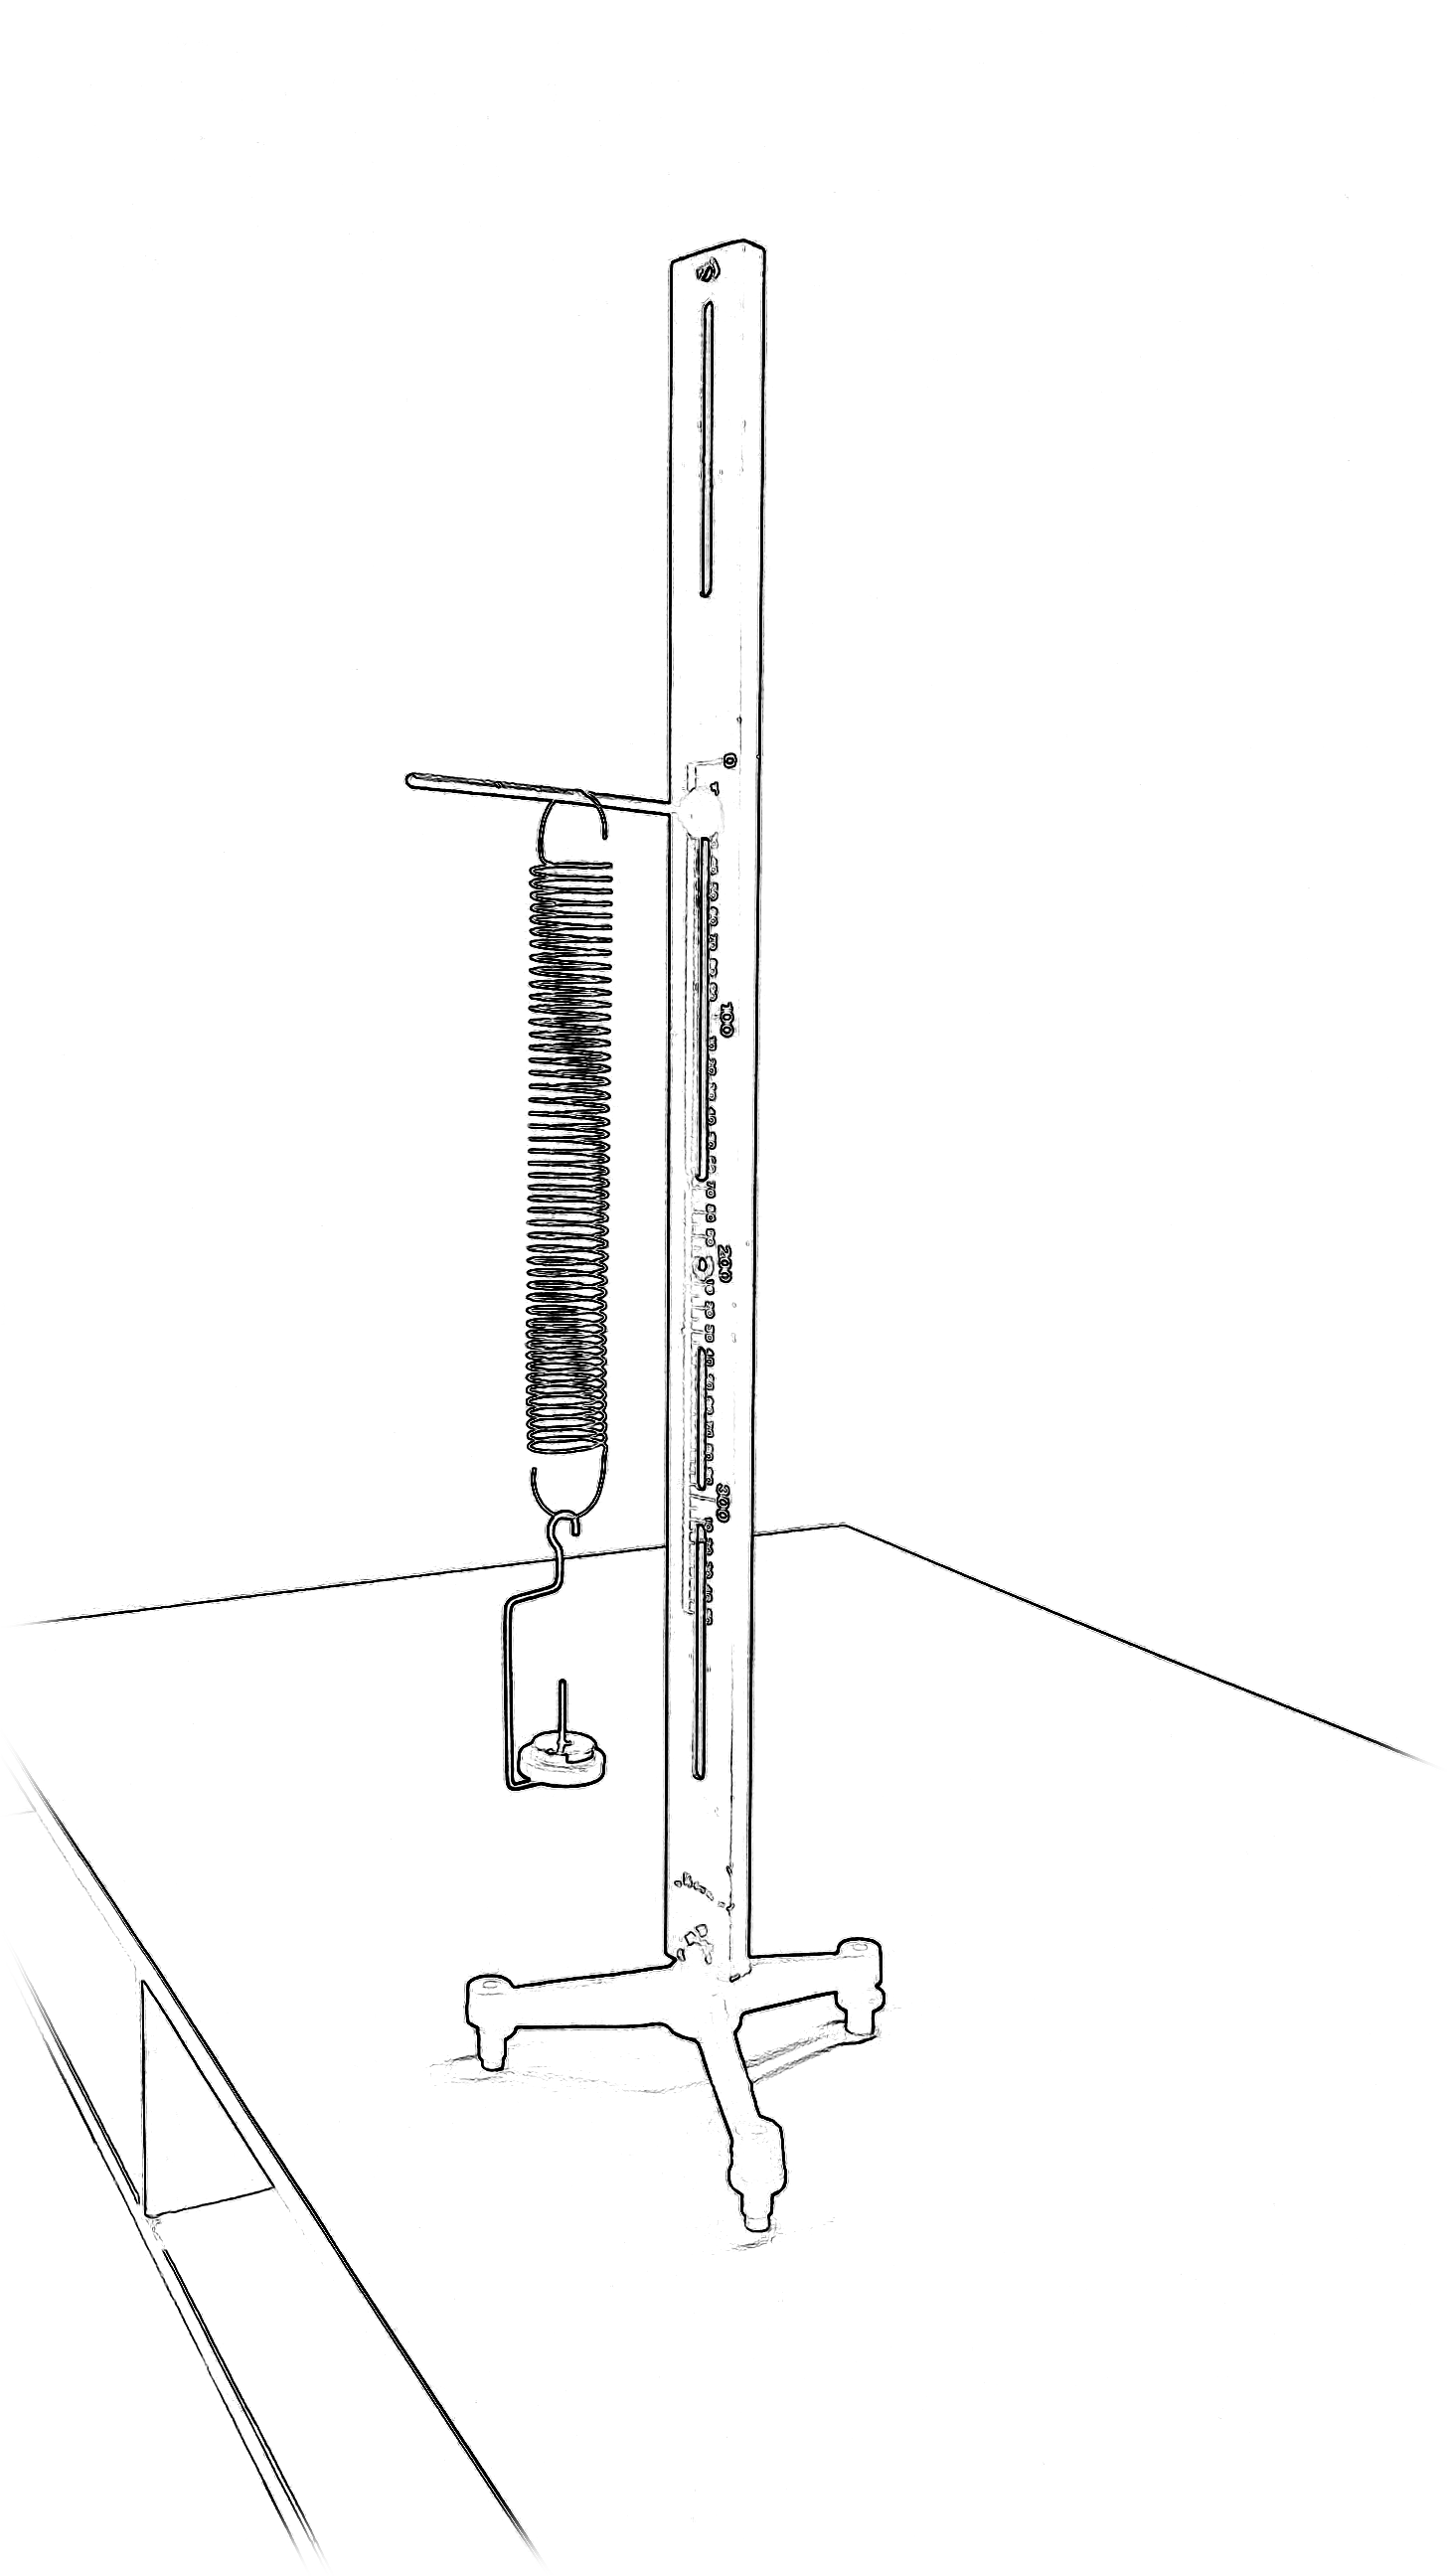
\includegraphics[width=\textwidth]{Ilustrations/Hooke.png}
\caption{Aparato para a verificação da distensão de um mola em função da massa por ela suportada.\label{Fig:IlustracaoLeiDeHooke}}
\end{marginfigure}

\begin{marginfigure}
\centering
\begin{tikzpicture}[>=Stealth]

    \draw[dashed, ->] (0,-1.5) -- (0,1.5) node[below left]{$y$};

	\draw[fill] (0,0) circle[radius = 0.1];
	\draw[->] (0,0) -- node[right]{$\vec{F}_e$}(0,1);
	\draw[->] (0,0) -- node[right]{$\vec{P}$}(0,-1);
	
\end{tikzpicture}
\caption{Diagrama de corpo livre para o corpo sustentado pela mola quando em equilíbrio.}
\label{DiagramaCorpoLivre}
\end{marginfigure}

Para uma mola, se realizarmos o mesmo procedimento, verificamos que ele sofre uma distensão \emph{distensão} gradual à medida que sustenta um peso maior. Fazendo um \emph{diagrama de corpo livre} (Figura~\ref{DiagramaCorpoLivre}), sabendo ainda que a aceleração do sistema é zero em uma condição de equilíbrio, concluímos que a força exercida pela mola sobre a caixa é igual em módulo e tem direção contrária à força peso da caixa (juntamente com sua carga):
\begin{align}
    F_{R, y} &= ma_y \\
    F_{e,y} + P_y &= 0 \\
    F_e - P &= 0 \\
	F_e &= P.
\end{align}

\pagebreak

\begin{marginfigure}
\centering
\begin{tikzpicture}[>=Stealth,
     interface/.style={
        % superfície
        postaction={draw,decorate,decoration={border,angle=-45,
                    amplitude=0.2cm,segment length=2mm}}},
    ]
    
    \draw[interface] (1,0) -- (-1,0);
    \draw[gray] (0,0) -- (0,-0.2);
    \draw[fill] (0,0) circle (1pt);
            
    \draw[decoration={aspect=0.3, segment length=0.8mm, amplitude=2mm,coil},decorate] (0,-0.2) -- +(0,-1);
    \draw[gray] (0,-1.2) -- (0,-1.4);
    \draw[fill] (0,-1.2) circle (1pt);
    
    \draw[<->|] (-0.5,0) -- node[left]{$L_0$} (-0.5,-1.2);
    \draw[densely dotted] (-0.5,-1.2) -- (0,-1.2);
        
    \begin{scope}[shift={(2.5,0)}]
        \draw[interface] (1,0) -- (-1,0);
        
        \draw[gray] (0,0) -- (0,-0.2);
        \draw[fill] (0,0) circle (1pt);
        
        \draw[decoration={aspect=0.3, segment length=1.5mm, amplitude=2mm,coil},decorate] (0,-0.2) -- +(0,-2);
        \draw[gray] (0,-2.2) -- (0,-2.4);
        \draw[fill] (0,-2.2) circle (1pt);
        
        \draw[densely dotted, pattern = north west lines] (-0.5, -2.4) rectangle (0.5,-3.4);
        \draw[<->|] (-0.5,0) -- node[left]{$L_0 + \Delta L$} (-0.5,-2.2);
        \draw[densely dotted](-0.5,-2.2) -- (0,-2.2);
        
%        \draw[fill] (0,-2.9) circle (1pt);
%        \draw[->, thick] (0, -2.9) -- +(0,-1) node[right]{$\vec{P}$};
%        \draw[->, thick] (0, -2.4) -- +(0,1) node[right, xshift=2mm]{$\vec{F}_e$};
        
%        \draw[dashed,->] (-0.75,-4.9) -- (-0.75,-0.9) node[below left]{$y$};
        
    \end{scope}
    
\end{tikzpicture}
\caption{A distensão $\Delta L$ da mola é proporcional à força elástica exercida por ela.}
\end{marginfigure}

Verificando ainda a distensão $\Delta L$ da mola, podemos relacionar uma maior distensão a uma carga maior na caixa, isto é, quanto maior a força peso dos objetos pendurados na mola, maior a distensão. Experimentalmente, verifica-se que a relação entre o peso aplicado à mola e sua distensão são \emph{diretamente proporcionais}:
\begin{equation}
	\Delta L \propto P.
\end{equation}

Podemos então escrever para o módulo da \textbf{força elástica} $F_e$
\begin{equation}
	F_e \propto \Delta L.
\end{equation}
%
Podemos escrever a relação acima como uma igualdade introduzindo uma constante de proporcionalidade $k$:
\begin{equation}\label{Eq:LeiDeHookeEmModulo}
	F_e = k \Delta L.
\end{equation}

O resultado acima é conhecido como \emph{Lei de Hooke}, em homenagem ao físico inglês Robert Hooke, que o verificou em 1660. Tal relação, no entanto, só é válida para um intervalo de distensões da mola. As distensões dentro deste limite são denominadas \emph{elásticas} e não deformam a mola permanentemente, caso contrário ao das distensões \emph{plásticas}. Apesar de a validade da Lei de Hooke ser limitada, ela é o modelo mais comum ao se analisar a resposta de um meio a uma deformação e pode ser utilizada como uma primeira aproximação mesmo para casos mais complexos.

Outro ponto que devemos considerar é o que acontece quando \emph{comprimimos} a mola. Se exercermos uma força conhecida, é possível verificar experimentalmente que a distensão sofrida pela mola segue a mesma relação linear dada pela Equação~\eqref{Eq:LeiDeHookeEmModulo}, com a mesma constante de proporcionalidade. Se considerarmos que a mola é helicoidal ---~como a mostrada na Figura~\ref{Fig:IlustracaoLeiDeHooke}~---, sendo que executamos deslocamentos somente na direção do próprio eixo da mola, podemos escrever uma relação vetorial que denota a direção e o sentido da força tanto para o caso da distensão, quanto para o caso da compressão da mola:
\begin{equation}
    \vec{F}_e = - k \vec{\Delta r}.
\end{equation}
%
Note que o sinal negativo implica em uma força que tem sempre o sentido oposto àquele que submetemos a mola, ou seja, a mola sempre exerce uma força no sentido de \emph{restaurar seu comprimento original}.\footnote{ Devido a isso, a força elástica denominada como uma \emph{força restauradora}.} Se optarmos por usar um sistema de referência, podemos colocar um dos eixos na direção do eixo da própria mola. Se nomearmos tal eixo como $x$, temos que
\begin{align}
    F_{e,x} &= -k \Delta x \\
    F_e &= -k \Delta x, \label{Eq:LeiDeHookeComoTodosConhecemos}
\end{align}
%
onde usamos o fato de que o vetor $\vec{F}_{e}$ aponta diretamente na direção de $x$, o que implica em $F_{e,x} \equiv F_e$ e $\Delta x$ representa a projeção do vetor $\Delta \vec{r}$ na direção do eixo $x$.\footnote[][-1cm]{Note que se $\Delta \vec{r}$ aponta na direção do eixo $x$, então $\Delta r = |\Delta \vec{r}| \equiv \Delta x$, mas a notação que todo mundo utiliza é a da Equação~\eqref{Eq:LeiDeHookeComoTodosConhecemos}. Só estou mostrando de onde essa forma vem.}

%%%%%%%%%%%%%%%%%%%%%%%%%%%%%%%%%%%%%%%%%%%%%
%\subsection{Se necessário, usar subsections}
%%%%%%%%%%%%%%%%%%%%%%%%%%%%%%%%%%%%%%%%%%%%%

%%%%%%%%%%%%%%%%%%%%%%%%%%%%%%%%%%%%%%%%%%%%%%%%%%%%%%%%%%%%%%%%%%%%%%%%%%%%%%%%%%%%%%%%
\section{Experimento: Determinação da distensão de uma mola em função da massa suspensa}
%%%%%%%%%%%%%%%%%%%%%%%%%%%%%%%%%%%%%%%%%%%%%%%%%%%%%%%%%%%%%%%%%%%%%%%%%%%%%%%%%%%%%%%%

Visando verificar a Lei de Hooke, vamos determinar a distensão de uma mola helicoidal posicionada verticalmente em função da massa de um conjunto de anilhas sustentada pela mola e em repouso. As anilhas serão ligadas à mola através de um gancho, permitindo que as depositemos uma a uma, verificando a distensão obtida para cada valor de massa suspensa. Note que devemos tomar o cuidado de verificar a distensão da mola sempre quando as anilhas suspensas se encontram em equilíbrio.

%%%%%%%%%%%%%%%%%%%%%%
\subsection{Objetivos}
%%%%%%%%%%%%%%%%%%%%%%

\begin{itemize}
     \item Verificar a lineariedade da distensão de uma mola em resposta à força peso dos objetos pendurados nela.
	 \item Relacionar as variáveis da Lei de Hooke às da equação da reta $y = A + Bx$.
     \item Calcular a constante $k$ da mola;
     \item Elaborar um gráfico $F_e \times \Delta x$ dos pontos experimentais e adicionar a ele a reta calculada através da regressão linear;
\end{itemize}

%%%%%%%%%%%%%%%%%%%%%%%%%%%%%%%%%%%%%%%%%%%%%%%%%%%%%%%%%%%%%%%%%%%%%%%%%%%%%%%
\section{Material Necessário}
%%%%%%%%%%%%%%%%%%%%%%%%%%%%%%%%%%%%%%%%%%%%%%%%%%%%%%%%%%%%%%%%%%%%%%%%%%%%%%%

\begin{itemize}
	\item Suporte vertical graduado com base e travessa horizontal;
	\item Molas diversas;
	\item Gancho e anilhas;
	\item Balança;
	\item Régua.
\end{itemize}

%%%%%%%%%%%%%%%%%%%%%%%%%%%%%%%%%%%%%%%%%%%%%%%%%%%%%%%%%%%%%%%%%%%%%%%%%%%%%%%
\section{Procedimento Experimental}
%%%%%%%%%%%%%%%%%%%%%%%%%%%%%%%%%%%%%%%%%%%%%%%%%%%%%%%%%%%%%%%%%%%%%%%%%%%%%%%

\begin{marginfigure}
\centering
\begin{tikzpicture}[>=Stealth,
     interface/.style={
        % superfície
        postaction={draw,decorate,decoration={border,angle=-45,
                    amplitude=0.2cm,segment length=2mm}}},
    ]
    
    \draw[interface] (1,0) -- (-1,0);
    \draw[gray] (0,0) -- (0,-0.2);
    \draw[fill] (0,0) circle (1pt);
            
    \draw[decoration={aspect=0.3, segment length=0.8mm, amplitude=2mm,coil},decorate] (0,-0.2) -- +(0,-1);
    \draw[gray] (0,-1.2) -- (0,-1.4);
    \draw[fill] (0,-1.2) circle (1pt);
    
    \draw[<->|] (-0.5,0) -- node[left]{$L_0$} (-0.5,-1.2);
    \draw[densely dotted] (-0.5,-1.2) -- (0,-1.2);
        
    \begin{scope}[shift={(2.5,0)}]
        \draw[interface] (1,0) -- (-1,0);
        
        \draw[gray] (0,0) -- (0,-0.2);
        \draw[fill] (0,0) circle (1pt);
        
        \draw[decoration={aspect=0.3, segment length=1.5mm, amplitude=2mm,coil},decorate] (0,-0.2) -- +(0,-2);
        \draw[gray] (0,-2.2) -- (0,-2.4);
        \draw[fill] (0,-2.2) circle (1pt);

        \draw[<->|] (-0.5,0) -- node[left]{$L$} (-0.5,-2.2);
        \draw[densely dotted](-0.5,-2.2) -- (0,-2.2);

        \draw[very thick, gray] ([shift=(-45:2mm)]0,-2.6) arc (-45:225:2mm) -- (-0.5,-3.5) -- (-0.5,-5.5) -- (0.5,-5.5) -- (0.5,-4);
        
        \fill[white] (-0.2,-5.48) rectangle (1.2, -5.1);
        \draw[gray, pattern = north west lines, pattern color = gray] (-0.2,-5.48) rectangle (1.2, -5.1);
        
               
%        \draw[fill] (0,-2.9) circle (1pt);
%        \draw[->, thick] (0, -2.9) -- +(0,-1) node[right]{$\vec{P}$};
%        \draw[->, thick] (0, -2.4) -- +(0,1) node[right, xshift=2mm]{$\vec{F}_e$};
        
%        \draw[dashed,->] (-0.75,-4.9) -- (-0.75,-0.9) node[below left]{$y$};
        
    \end{scope}
    
\end{tikzpicture}
\caption{Para que possamos determinar o valor de $\Delta L$, devemos escolher dois pontos \emph{fixos} de referência. Note que $\Delta L = L - L_0$.\label{Fig:LeiDeHookeMolaPontosDeRef}}
\end{marginfigure}
\begin{enumerate}
	\item Utilize o suporte para fixar a mola por uma extremidade e prenda o gancho à outra extremidade.
	\item Marque dois pontos de referência,\footnote[][1cm]{Como estamos interessados em determinar a distensão $\Delta L$ da mola, quaisquer dois pontos que permitam determinar tal valor são adequados. Podemos, por exemplo, colocar o ponto mais baixo na parte inferior do gancho, uma vez que a altura do gancho é constante e não influi no valor de $\Delta L$.}  um na parte superior e outro na parte inferior da mola (veja a Figura~\ref{Fig:LeiDeHookeMolaPontosDeRef}). Meça a distância $L_0$ entre eles e anote na Tabela~\ref{Dados}.
	\item Verifique a massa de uma anilha, juntamente com o gancho, e os suspenda na mola. Verifique a nova distância $L$ entre os pontos de referência. Anote  na Tabela~\ref{Dados} os valores da massa suspensa $m_s$ e a distância $L$ obtidas.
	\item Afira a massa de outra anilha e a coloque no gancho. Verifique a nova distância $L$ entre os pontos de referência. Anote na Tabela~\ref{Dados} o novo valor da massa suspensa $m_s$ e o novo valor da distância $L$.
	\item Repita o passo acima adicionando anilhas ao gancho uma a uma. Procure conseguir o máximo número de pontos experimentais possível, porém sem submeter a mola a deformações irreversíveis.
\end{enumerate}

%%%%%%%%%%%%%%%%%%%%%%%%%%%%%%%%%%%%%%%%%%%%%%%%%%%%%%%%%%%%%%%%%%%%%%%%%%%%%%%
%%%%%%%%%%%%%%%%%%%%%%%%%%%%%%%%%%%%%%%%%%%%%%%%%%%%%%%%%%%%%%%%%%%%%%%%%%%%%%%
%%%%%%%%%%%%%%%%%%%%%%%%%%%%%%%%%%%%%%%%%%%%%%%%%%%%%%%%%%%%%%%%%%%%%%%%%%%%%%%
%%%%%%%%%%%%%%%%%%%%%%%%%%%%%%%%%%%%%%%%%%%%%%%%%%%%%%%%%%%%%%%%%%%%%%%%%%%%%%%
\cleardoublepage

\noindent{}{\huge\textit{Lei de Hooke}}

\vspace{15mm}

\begin{fullwidth}
\noindent{}\makebox[0.6\linewidth]{Turma:\enspace\hrulefill}\makebox[0.4\textwidth]{  Data:\enspace\hrulefill}
\vspace{5mm}

\noindent{}\makebox[0.6\linewidth]{Aluno(a):\enspace\hrulefill}\makebox[0.4\textwidth]{  Matrícula:\enspace\hrulefill}

\noindent{}\makebox[0.6\linewidth]{Aluno(a):\enspace\hrulefill}\makebox[0.4\textwidth]{  Matrícula:\enspace\hrulefill}

\noindent{}\makebox[0.6\linewidth]{Aluno(a):\enspace\hrulefill}\makebox[0.4\textwidth]{  Matrícula:\enspace\hrulefill}

\noindent{}\makebox[0.6\linewidth]{Aluno(a):\enspace\hrulefill}\makebox[0.4\textwidth]{  Matrícula:\enspace\hrulefill}

\noindent{}\makebox[0.6\linewidth]{Aluno(a):\enspace\hrulefill}\makebox[0.4\textwidth]{  Matrícula:\enspace\hrulefill}
\end{fullwidth}

\vspace{5mm}

%%%%%%%%%%%%%%%%%%%%%%%%%%%%%%%%%%%%%%%%%%%%%%%%%%%%%%%%%%%%%%%%%%%%%%%%%%%%%%%
\section{Questionário}
%%%%%%%%%%%%%%%%%%%%%%%%%%%%%%%%%%%%%%%%%%%%%%%%%%%%%%%%%%%%%%%%%%%%%%%%%%%%%%%

\begin{question}[type={exam}]{1}
Apresente os resultados de maneira clara e organizada. Mostre os cálculos requisitados de maneira clara e sucinta, evidenciando o raciocínio desenvolvido.
\end{question}

\begin{question}[type={exam}]{2}
Preencha as colunas de dados experimentais das tabelas com o número adequado de algarismos significativos e unidades.
\end{question}

\begin{question}[type={exam}]{1} 
Calcule a constante $k$ da mola, para cada conjunto de valores de peso\footnote{O peso deve ser calculado através do produto dos valores de massa suspensa $m_s$ pela aceleração da gravidade $g$.} e distensão.
\end{question}

\begin{question}[type={exam}]{1} 
Relacione as variáveis da Lei de Hooke àquelas da equação da reta e inteprete o significado das constante $A$ e $B$.
\end{question}

\begin{question}[type={exam}]{2} 
Determine a constante da mola através da regressão linear.
\end{question}

\begin{question}[type={exam}]{2} 
Elabore um gráfico de\footnote{Apesar de o mais adequado ser um gráfico de $\Delta x \times m$, pois controlamos a massa suspensa ($m$ é, portanto, a variável independente) e medimos a distensão correspondente da mola ($\Delta x$ é então a variável dependente), para fins didáticos é melhor elaborarmos um gráfico de  $F_e \times \Delta x$.} $F_e \times \Delta x$ para os dados experimentais obtidos e adicione a ele a reta calculada através da regressão linear.
\end{question}

\begin{question}[type={exam}]{1} 
Determine o valor de $r^2$. O valor encontrado demonstra compatibilidade entre os dados experimentais e a hipótese de dependência linear da distensão com a força aplicada à mola?
\end{question}
\vfill

%%%%%%%%%%%%%%%%%%%%%%%%%%%%%%%%%%%%%%%%%%%%%%%%%%%%%%%%%%%%%%%%%%%%%%%%%%%%%%%
\pagebreak
\section{Tabelas}
%%%%%%%%%%%%%%%%%%%%%%%%%%%%%%%%%%%%%%%%%%%%%%%%%%%%%%%%%%%%%%%%%%%%%%%%%%%%%%%

\begin{table}
\centering
\begin{tabular}{lp{25mm}p{25mm}p{25mm}l}
\toprule
	& \multicolumn{3}{l}{\textbf{Dados Experimentais}} \\
	\cmidrule{2-3}
	& \cellcolor[gray]{0.89} $L_0$ & \cellcolor[gray]{0.92} \\
	\cmidrule{2-3}
	\\
	\cmidrule{2-3}
	& $L$ & $m_s$ & \\
	\cmidrule{2-3}
	& \cellcolor[gray]{0.89} & \cellcolor[gray]{0.92} \\
	& \cellcolor[gray]{0.95} & \cellcolor[gray]{0.97} \\
	& \cellcolor[gray]{0.89} & \cellcolor[gray]{0.92} \\
	& \cellcolor[gray]{0.95} & \cellcolor[gray]{0.97} \\
	& \cellcolor[gray]{0.89} & \cellcolor[gray]{0.92} \\
	& \cellcolor[gray]{0.95} & \cellcolor[gray]{0.97} \\
	& \cellcolor[gray]{0.89} & \cellcolor[gray]{0.92} \\
	& \cellcolor[gray]{0.95} & \cellcolor[gray]{0.97} \\
	& \cellcolor[gray]{0.89} & \cellcolor[gray]{0.92} \\
	& \cellcolor[gray]{0.95} & \cellcolor[gray]{0.97} \\
	& \cellcolor[gray]{0.89} & \cellcolor[gray]{0.92} \\
	& \cellcolor[gray]{0.95} & \cellcolor[gray]{0.97} \\
	\cmidrule{2-4}
\\
	& \multicolumn{3}{l}{\textbf{Valores calculados}} \\
	\cmidrule{2-4}
	& $|\Delta x|$ & $P$ & $k = P/\Delta x$ \\
	\cmidrule{2-4}
	& \cellcolor[gray]{0.89} & \cellcolor[gray]{0.92} & \cellcolor[gray]{0.89} \\
	& \cellcolor[gray]{0.95} & \cellcolor[gray]{0.97} & \cellcolor[gray]{0.95} \\
	& \cellcolor[gray]{0.89} & \cellcolor[gray]{0.92} & \cellcolor[gray]{0.89} \\
	& \cellcolor[gray]{0.95} & \cellcolor[gray]{0.97} & \cellcolor[gray]{0.95} \\
	& \cellcolor[gray]{0.89} & \cellcolor[gray]{0.92} & \cellcolor[gray]{0.89} \\
	& \cellcolor[gray]{0.95} & \cellcolor[gray]{0.97} & \cellcolor[gray]{0.95} \\
	& \cellcolor[gray]{0.89} & \cellcolor[gray]{0.92} & \cellcolor[gray]{0.89} \\
	& \cellcolor[gray]{0.95} & \cellcolor[gray]{0.97} & \cellcolor[gray]{0.95} \\
	& \cellcolor[gray]{0.89} & \cellcolor[gray]{0.92} & \cellcolor[gray]{0.89} \\
	& \cellcolor[gray]{0.95} & \cellcolor[gray]{0.97} & \cellcolor[gray]{0.95} \\
	& \cellcolor[gray]{0.89} & \cellcolor[gray]{0.92} & \cellcolor[gray]{0.89} \\
	& \cellcolor[gray]{0.95} & \cellcolor[gray]{0.97} & \cellcolor[gray]{0.95} \\
	\cmidrule{2-4}
\bottomrule
\end{tabular}
\caption{Valores de posição em função da massa pendurada na mola.}
\label{Dados}
\end{table}
